\section{Parameter estimation and Bayesian lens reconstruction}
\label{sec:pe}
The benchmark of Sec.~\ref{sec:results} uses a simplified, SNR-based model of the GW measurements (Sec.~\ref{sec:gwmeas}) and estimators trained on simulations. Here we test both ingredients on a random subset of systems, with equal numbers per lens family and scenario: the SNR-based model against joint Bayesian parameter estimation (PE) of both images from simulated detector data (strain), and the trained estimators against a conventional Bayesian lens reconstruction from comparable observables. The information available to each method is stated explicitly below, because it is not identical.

\subsection{Joint parameter estimation of lensed image pairs}
\label{sec:jointpe}
We drew 15 selected systems per lens family and scenario (120 in total) at random from catalogs generated with the same configuration as the benchmark, excluding the lightest detector-frame binaries whose analysis segment would exceed 256\,s. For each system both images were injected into independent stationary Gaussian noise with the A+/AdV (O5-like) or ET-D power spectral densities, using the \textsc{IMRPhenomXHM} waveform with higher harmonics \citep{garciaquiros2020xhm}, the Morse phase of each image and the antenna patterns at each arrival time. We sampled the joint posterior of the shared source parameters (chirp mass, mass ratio, aligned spins, sky position, polarization, inclination, phase, apparent distance and arrival time of image $A$) and the lensing parameters $\ln(\mu_B/\mu_A)$, the delay and the two Morse indices, with \textsc{bilby} \citep{ashton2019bilby}, the \textsc{dynesty} nested sampler \citep{speagle2020dynesty} and relative binning \citep{zackay2018relbin,krishna2023relbin}, which speeds up the likelihood by expanding each waveform around a reference waveform. In this controlled test the reference is the injected signal; for real data it would be a maximum-likelihood fit. Where the relative-binning log-likelihood exceeds that of the reference by more than 50, which signals a failure of the approximation because the reference lies close to the maximum-likelihood point, we evaluate the exact likelihood instead. This safeguard does not bound the error elsewhere, so we evaluated the exact likelihood on 500 posterior samples of every system whose stored samples allow it (all 60 ET and 52 of the 60 O5 systems; the stored samples of eight early O5 runs lack the phase) and reweighted the samples by the likelihood ratio. For O5 the difference is negligible (posterior shifts of $\ln(\mu_B/\mu_A)$ below $0.03\sigma$). For ET the log-likelihood differences have a typical scatter of 0.27; reweighting shifts the median of $\ln(\mu_B/\mu_A)$ by a median $0.01\sigma$ (at most $0.10\sigma$) and that of $\ln D_{{\rm app},A}$ by $0.03\sigma$ (at most $0.25\sigma$), changes interval widths by less than 10\% for the magnification ratio, and leaves its coverage unchanged. We analyzed every system twice: with a free sky position, as in a GW-only analysis, and with the sky position fixed to that of the host, which is known to sub-arcsecond precision once the lens system is identified in imaging, as the benchmark assumes. The apparent-distance prior is uniform in volume. We used 150 live points and the acceptance-walk method of \textsc{bilby}, with 30 accepted Markov-chain steps for each new live point. For the free-sky ET posteriors, which have several separated solutions, these settings do not explore all of them (see below), which is one reason we base the comparison with the SNR-based model on the known-sky analyses. Each system has its own noise realization, fixed by a seed derived from its identifier, so that the GW-only and GW+EM analyses below see identical data. A run takes of order 10--30 CPU hours.

Fig.~\ref{fig:pe} compares the joint-PE posteriors with the SNR-based model of Sec.~\ref{sec:gwmeas}. With the host sky position, the 90\% intervals of $\ln(\mu_B/\mu_A)$ and of the apparent distance of image $A$ contain the truth for 52 and 50 of the 60 ET systems (coverage $0.87\pm0.04$ and $0.83\pm0.05$, binomial errors), and the free-sky O5 intervals for 55 and 53 of 60 ($0.92\pm0.04$ and $0.88\pm0.04$). The probability integral transforms are consistent with uniform (Kolmogorov--Smirnov $p=0.06$ for ET and $0.09$ for O5), and the difference of Morse indices is identified with posterior probability above 0.5 in all ET and in 59 of 60 O5 systems. For the tested systems the PE uncertainties are smaller than those of the SNR-based model: by a factor 0.91 for $\ln(\mu_B/\mu_A)$ in O5 and 0.41 in ET, and by factors 0.67 and 0.44 for $\ln D_{{\rm app},A}$. In these comparisons the SNR-based model is therefore conservative, especially for ET. The joint PE fixes the source parameters that the two images share, and the higher harmonics break part of the inclination--distance degeneracy that dominates the catalog-calibrated apparent-distance errors, so the median $\sigma_{\ln D}$ is 0.10 for ET rather than 0.24.

Free-sky ET analyses fail in a characteristic way. A single ET site constrains the sky position poorly, and the sky position, the polarization and the Morse phase of each image are partly degenerate. With 150 live points the median sky offset is $56\degr$, the Morse-index difference is identified in only 82\% of systems, and the coverage of $\ln(\mu_B/\mu_A)$ falls to 0.67. With 500 live points the coverage rises only to 0.75, and for the 15 systems whose intervals still miss the truth the posterior favors other sky positions, so these failures are a property of single-site data rather than of the sampler. Fixing the sky position to that of the identified host, which is available whenever the lens is identified, removes them. O5 analyses, with three detectors, are not affected.

As a test of the complete chain from detector data to magnification, we replaced the simulated magnification ratio in the input of the scale-free Geometry\,+\,$\mu$ ratio\,+\,$z,\sigma_v$ NPE by the PE posterior median and kept the per-family conformal calibration of Sec.~\ref{sec:calibration}. The median relative error of $\mu_A$ is 10.5\% for ET with the host sky position (10.8\% with the SNR-based model) and 13.8\% for O5 (17.8\%), with coverage 0.85 and 0.87 for both inputs. The NPE trained with the SNR-based model therefore works with relative magnifications measured by full PE. The SIS intervals under-cover in this subset (0.67--0.73 of 15 systems) for both inputs; these intervals are only a few percent wide, and the test-set coverage for SIS is nominal, so we attribute this to the small sample.

\begin{figure*}
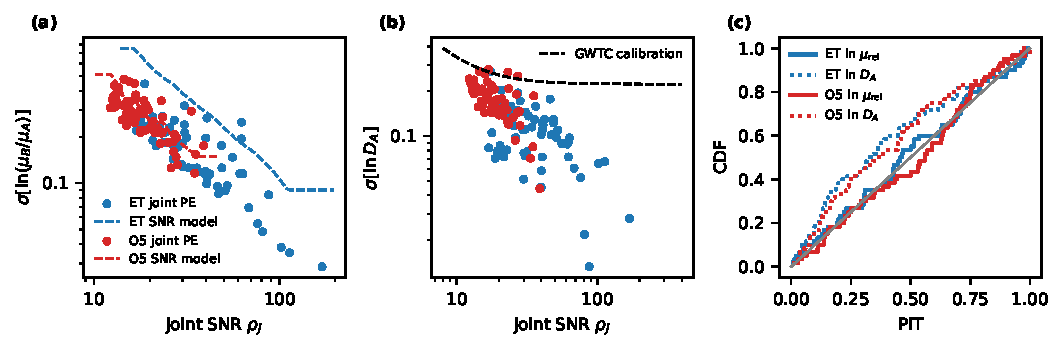
\includegraphics[width=\textwidth]{figures/fig_pe.pdf}
\caption{Joint PE of 120 lensed image pairs from simulated strain. (a) Posterior standard deviation of $\ln(\mu_B/\mu_A)$ versus joint network SNR, with the SNR-based model (dashed). (b) The same for the apparent distance of image $A$, with the GWTC-calibrated error model. (c) Distribution of the probability integral transforms of the truth (diagonal: perfect calibration). ET uses the host sky position, O5 a free sky position.}
\label{fig:pe}
\end{figure*}

\subsection{Bayesian GW+EM lens reconstruction}
\label{sec:gwem}
For the same systems we reconstructed the lens with a conventional likelihood, specified in Appendix~\ref{app:gwemlike}. The lens model is the simulated family (SIS, SIE, SIE+shear or EPL+shear), evaluated with \textsc{lenstronomy}, and its priors are the simulated population distributions: the SLACS-like axis ratio, the log-normal external shear, $\gamma'\sim\mathcal N(2.08,0.15)$ and the $\sigma_v^4$-weighted velocity-dispersion function. The EM likelihood contains the image positions, with the source position integrated out analytically after linearizing the lens equation around each observed image, the lens-light axis ratio and orientation, the velocity dispersion through the SIS normalization, and the lens-light center. The prior of the source position is normalized for each lens as in the simulation; without this normalization the fit favors steep radial profiles (Appendix~\ref{app:gwemlike}). The GW data enter through the joint-PE posterior of Sec.~\ref{sec:jointpe}, summarized by a Gaussian in $\ln(\mu_B/\mu_A)$ after reweighting the samples to remove the distance prior and multiplied by the posterior probabilities of the nine Morse-index combinations, analogous to the effective GW likelihood of \citet{uronen2026silmarel}. The product is sampled over the lens parameters with 500 live points. For 79 of the systems we also sampled the strain and EM likelihoods together, with all source parameters free; the posterior medians of $\ln\mu_A$ from the two analyses differ by a median $0.15\sigma$ (ET) and $0.05\sigma$ (O5), where $\sigma$ is the posterior width, and the interval widths agree, so the summary of the GW posterior is adequate (details will be given in a companion paper).

No cosmology is assumed. The GW amplitude then constrains only the magnification ratio, and only the arrival order of the delay is used, so the analysis uses the observables of the scale-free Geometry\,+\,$\mu$ ratio\,+\,$z,\sigma_v$ combination. It differs from the NPE in two respects: it also uses the Morse indices, and it assumes the simulated lens family, whereas the NPE is trained on a mixture of all four families. To remove the knowledge of the family, we repeated the analysis with the EPL+shear model for every system. One O5 system is excluded because its catalog entry could not be reproduced exactly from the stored inputs.

Table~\ref{tab:gwem} compares the two methods. With the simulated lens family and, for ET, the host sky position, the Bayesian analysis determines $\mu_A$ to a median 7.9\% for ET and 13.7\% for O5. The NPE, given the same PE magnification ratio but neither the family nor the Morse indices, reaches 10.5 and 13.8\%. With the EPL+shear model for every system the Bayesian errors rise to 12.4 and 18.6\%; without the normalization of the source-position prior they would be 16.2 and 20.6\%. The two methods thus achieve comparable point-estimate errors when the Bayesian analysis knows the family; without that knowledge, the NPE's prior, a mixture of the simulated families, is more informative than a single flexible model, as long as the simulated population is correct.

The Bayesian intervals are 40--45\% narrower than those of the NPE but contain the truth less often: for 0.82 (ET) and 0.92 (O5) of the systems, against 0.85 and 0.87 for the NPE, with binomial errors of about 0.04. The ET shortfall of about $2\sigma$ is not caused by the linearized position likelihood, because the exact likelihood of Appendix~\ref{app:gwemlike} gives 0.83. Nominal 90\% Bayesian intervals should therefore not be read as calibrated without such checks. With the EPL+shear model the coverage is 0.95 (ET) and 0.88 (O5); these intervals are not corrected, so they should not be compared with the conservative transfer of the calibrated estimators in Sec.~\ref{sec:transfer}.

\begin{table}
\caption{Bayesian GW+EM reconstruction and NPE for the same systems: median relative error of $\mu_A$ and coverage of the 90\% interval, for 60 systems per scenario (59 for the O5 Bayesian analyses). No cosmology is assumed. ET uses the host sky position, O5 a free sky position. The NPE uses the scale-free Geometry\,+\,$\mu$ ratio\,+\,$z,\sigma_v$ observables, with the magnification ratio from the SNR-based model or from joint PE.}
\label{tab:gwem}
\begin{tabular*}{\linewidth}{@{\extracolsep{\fill}}lcccc@{}}
\toprule
 & \multicolumn{2}{c}{ET} & \multicolumn{2}{c}{O5} \\
Analysis & err. (\%) & cov. & err. (\%) & cov. \\
\midrule
Bayesian, simulated family & 7.9 & 0.82 & 13.7 & 0.92 \\
Bayesian, EPL+shear for all & 12.4 & 0.95 & 18.6 & 0.88 \\
NPE, SNR-model $\mu_B/\mu_A$ & 10.8 & 0.85 & 17.8 & 0.87 \\
NPE, joint-PE $\mu_B/\mu_A$ & 10.5 & 0.85 & 13.8 & 0.87 \\
\bottomrule
\end{tabular*}
\end{table}
